\documentclass{sigkddExp}

%%%%%%%%%%%%%%%%%%%%%%%%%%%%%%%%%%%%%%%%%%%%%%%%%%%%%%%%%%
% TITLE
%%%%%%%%%%%%%%%%%%%%%%%%%%%%%%%%%%%%%%%%%%%%%%%%%%%%%%%%%%
%Title will probably change
\title{Predicting crime rates using taxi rides data}


%%%%%%%%%%%%%%%%%%%%%%%%%%%%%%%%%%%%%%%%%%%%%%%%%%%%%%%%%%
% AUTHORS
%%%%%%%%%%%%%%%%%%%%%%%%%%%%%%%%%%%%%%%%%%%%%%%%%%%%%%%%%%
\numberofauthors{3}
\author{
\alignauthor Carlos Petricioli \\
       % \affaddr{Computer Science Department}\\
       \affaddr{New York University}\\
       \affaddr{New York, USA}\\
       \email{petricioli@nyu.edu}
\alignauthor Valerie Angulo\\
       % \affaddr{Computer Science Department}\\
       \affaddr{New York University}\\
       \affaddr{New York, USA}\\
       \email{vaa238@nyu.edu}
\alignauthor Varsha Muralidharan \\
       % \affaddr{Computer Science Department}\\
       \affaddr{New York University}\\
       \affaddr{New York, USA}\\
       \email{vm1370@nyu.edu}
}


\begin{document}

\maketitle

%%%%%%%%%%%%%%%%%%%%%%%%%%%%%%%%%%%%%%%%%%%%%%%%%%%%%%%%%%
% ABSTRACT
%%%%%%%%%%%%%%%%%%%%%%%%%%%%%%%%%%%%%%%%%%%%%%%%%%%%%%%%%%
\begin{abstract}

Understanding and predicting crime is a crucial task in any major city. The ability to see patterns of criminal activity in certain areas is useful, but pairing crime data with geographic information present in taxi usage data adds depth to our understanding of crime and people's reactions to perceived danger in certain locations. The objective of this study is to understand crime rates at a granular level with the idea that people behave according to how secure they feel, which extends to travel preferences. It is inferred that people are less likely to walk or use public modes of transportation in areas subjectively deemed more dangerous, and will instead opt to use more reliable and immediate transportation such as designated taxis. New York City will be used in this study as it provides a large amount of public data on crimes throughout the five boroughs along with an extensive amount of data from NYC yellow cab usage. This is a modern approach that will complement the use of demographics and geographical variables commonly used to predict crime. Global Positioning System (GPS) data on taxi rides provide useful information that can be directly related to crime at a block level and weather data will be used as a secondary source to explain an inferred higher usage of taxis in undesirable weather conditions. 

\end{abstract}



%%%%%%%%%%%%%%%%%%%%%%%%%%%%%%%%%%%%%%%%%%%%%%%%%%%%%%%%%%
% INTRODUCTION
%%%%%%%%%%%%%%%%%%%%%%%%%%%%%%%%%%%%%%%%%%%%%%%%%%%%%%%%%%

\section{Introduction}

Crime is an important factor to consider for those working and living in an area. Usually people tend to want to live in areas they consider safe while minimizing time spent in locations considered unsafe. %CITATION OF THIS FACT. SOMEONE COULD ARGUE THAT PEOPLE RISK LIVING ON UNSEFURE PLACES ON CERTAIN
What goes into an individuals subjective view of what is safe versus unsafe can be hard to gage. However, a lot can be inferred from an individuals behavior patterns. One such pattern of behavior is transportation habits. We hope to correlate taxi pickup and drop off information to the perceived level of crime activity in an area. It is inferred that people choose to not use public modes of transportation in areas where an individual feels unsafe or uncomfortable and will instead opt to use a more direct and safer source such as a designated taxi. Through open source data of taxi trips, we hope to correlate peoples transportation behavior with the rate of crime activity in a given area. 


The area we are conducting this study on is New York City.
% WE SHOULD INCLUDE SOME CRIME FACTS AND HOW RELEVANT IS TO UDERNSANT IT. INCLUDE A QUICK COMPARATION TO OTHER MAYOR CITIES TO ARGUE THAT WE HAVE A PREFFERENCE FOR NYC FOR XXX REASON.


Our primary reason is that there are an abundance of transportation services available in New York City and taxi data is common enough to garner a big data set. 
%THIS IS NOT THEEEE PRIAMARY REASON ITS JUST CONVENIENT FOR US. THE PRIMARY REASON SHOULD BE THAT WE CONSIDER NYC INTERESTING FOR ITS BLAAA..., IT COULD BE ANYTHING BUT THERE ARE ABUNDANCE OF TRANSPORTANTION SERVICES IN MANY PLACES AND WE STILL PICKED NYC BECAUSE X.


% IN NOT SURE THIS IS ACUTALLY TRUE IF IT IS WE SHOULD CITE SOMETHING: 
       % It is also easy for individuals to choose a reliable taxi company, the NYC yellow taxi, which is a widely used and reputable taxi company. 
With the abundance of transportation options, our study can explore transportation patterns such as taxi usage versus subway usage based on subway locations and taxi pickup/drop off coordinates. %ITS NOT VS SUBWAY USAGE BECASE WE CANNOT BE SURE OF THAT. IT SHOULD BE SOMETHING LIKE TAXI USAGE GIVEN THE PROXIMITY TO A SUBWAY STATION AT A GIVEN LOCATION.

New York City also has an Open Data Law which mandates that all public crime data be available online \cite{OpenDat}. This has made crime data collection easily accessible to the public.

Relating crime to transportation is important because it uses the knowledge of those who live in an area to predict which areas may be more prevalent to crime. %I DONT LIKE THIS SENTENCE HAHA. 
This is an intuitive source of information that utilizes people and their knowledge of the city in crime prediction. %SAME HERE THIS IS A COMPLEX THING TO SAY WE SHOULD KEEP IT SIMPLE 

This study can give a look into what areas people avoid, allowing to geographically match the locations of crime activity to geographical pickup/drop off locations of taxi trips provided in the open source taxi data \cite{Taxi} and can also provide information into the development of areas that become more or less crime ridden. 

The data collected for this study contains historic \cite{NYPDHis} and current \cite{NYPDCur} records from NYPD complaint data, this is a historic and current representation of crime versus taxi usage patterns in New York City from 2006 until present. Data collected from NOAA \cite{NOAA} is used as a third data source in order to provide a more controlled analysis. Weather is used as a possible explanation for taxi/crime patterns that do not correlate, seeing as weather is often a factor in the decision to take certain forms of transportation.%% CITES HERE.

%NOT ACCURATE: For this study, we will compare the distance of taxi pickup locations to reported locations of crime activity. This is so that we can unite these two data sources based on geographic locations within the city. 


These three data sets were downloaded in the NYU cluster DUMBO and saved in HDFS, as shown in Figure \ref{figx}, in order to be cleaned and formatted before coding the analytic. Both crime and taxi data contain latitude and longitude data, which we have used to link the two data sources. 
We have performed a spatial join with the coordinates for crime activity and taxi usage to a specific  taxi zone ID representing a sub-area of New York City in order to have a commonly defined location between the two sources.
Hourly weather data collected at three points, Central Park, LaGuardia and JFK, was assigned to each taxi ride by picking the data collected from the nearest station to the pickup location at a given time. 

The first step in our analytic is to homogenize the crime and taxi data geographic locations in order to be able to compare the two data sets with one another. After relating the data sets in this way, we made sure that the time of each taxi pickup and crime event were correlated, all the while noting the hourly weather conditions in the general location of the taxi pickup/crime occurrence. From this information we were able to answer specific questions such as whether taxi pickup data suggested that some areas were less safe than others, how much of a part weather played in taxi usage, the general distance between pickup and drop off locations that would suggest a person would call a taxi and the rate of taxi usage compared to the distance of the nearest subway station. Many transportation patterns can be inferred by the three data sets. We inferred that an individual or group would use a taxi if the location was subjectively deemed unsafe, too far from the destination point or the individual or group was caught in weather that made other sources of transportation less appealing. 


%%%%%%%%%%%%%%%%%%%%%%%%%%%%%%%%%%%%%%%%%%%%%%%%%%%%%%%%%%
% BODY
%%%%%%%%%%%%%%%%%%%%%%%%%%%%%%%%%%%%%%%%%%%%%%%%%%%%%%%%%%
\section{BODY}
% body goes here

% \subsubsection{Equations}
% put any equations here

\subsection{Related Works}
There have been various studies on big data sources used in conjunction with crime data in order to understand and predict crime patterns. In one such study \cite{Wang16} the authors propose to use points of interest (POI) and taxi flow data in Chicago to make inferences on crime patterns. It is hypothesized that taxi flows are “hyper links” within a city that connect locations, where they may be a proxy for broader patterns of population routine activity and mobility, commuting flows, and other forms of social and economic exchanges between two communities over space. The authors use POI to enhance the demographics information and use taxi flow as hyper links to enhance the geographical proximity correlation however, the temporal dimension of crime is not considered in depth. The problem in this study is population-centric, where the crime rate for Chicago is profiled in community areas that are well-defined and stable geographical regions. The proposed POI features and taxi links provide new perspectives in profiling the crime rate across community areas and the crime data collected in Chicago contains detailed information about the time, location and type of crime committed.

Other studies utilize crowd sourced data to predict crime patterns. In a recent study \cite{Bendler14} crowd sourcing of tweets was used as a virtual neighborhood watch in order to find crime patterns. The rough location for where the twitter post was sent can be determined by the social network provider or by geo-tags from the users phone. This study inferred that there was a correlation between an important event and the amount of tweets traced to a specific area, where an increase in the amount of tweets in a given area within a certain time span suggests an event was occurring at that time and place. The goal of this study was to predict and explain crimes in urban areas through tweet volume where crime and tweets were related through time and location. This study collected tweets and crime data in hourly blocks at Market Street in San Fransisco during a duration of three months. 

Urban crime has been correlated with different modes of communication data as well \cite{Traunmueller14}. The authors of a recent study presented a method to relate crime in London and people dynamics through the utilization of crime data records for the area of Greater London and data from a mobile telecommunication provider for details of people dynamics. Crime data was recorded with latitude/longitude coordinates whereas the telecommunication data was available as footfall in grids of varying sizes (smaller grids in central London as opposed to larger grids in less densely populated areas outside central London). While many people dynamics were looked at in depth in regards to crime, there were two major limitations in the study performed. One was that the crime data was recorded on a monthly basis whereas the telecommunications data recorded footfall on an hourly basis. This limitation is avoided in our study by grouping the data together by hour so that it is more cohesive. Because our study emphasizes time and location of taxi usage, crime activity and surrounding weather conditions, we have made sure that our three data sources share these conditions.


\subsection{Design}
Figure \ref{figx} shows our data flow diagram.

\begin{figure}
\caption{Data flow diagram}
\label{figx}
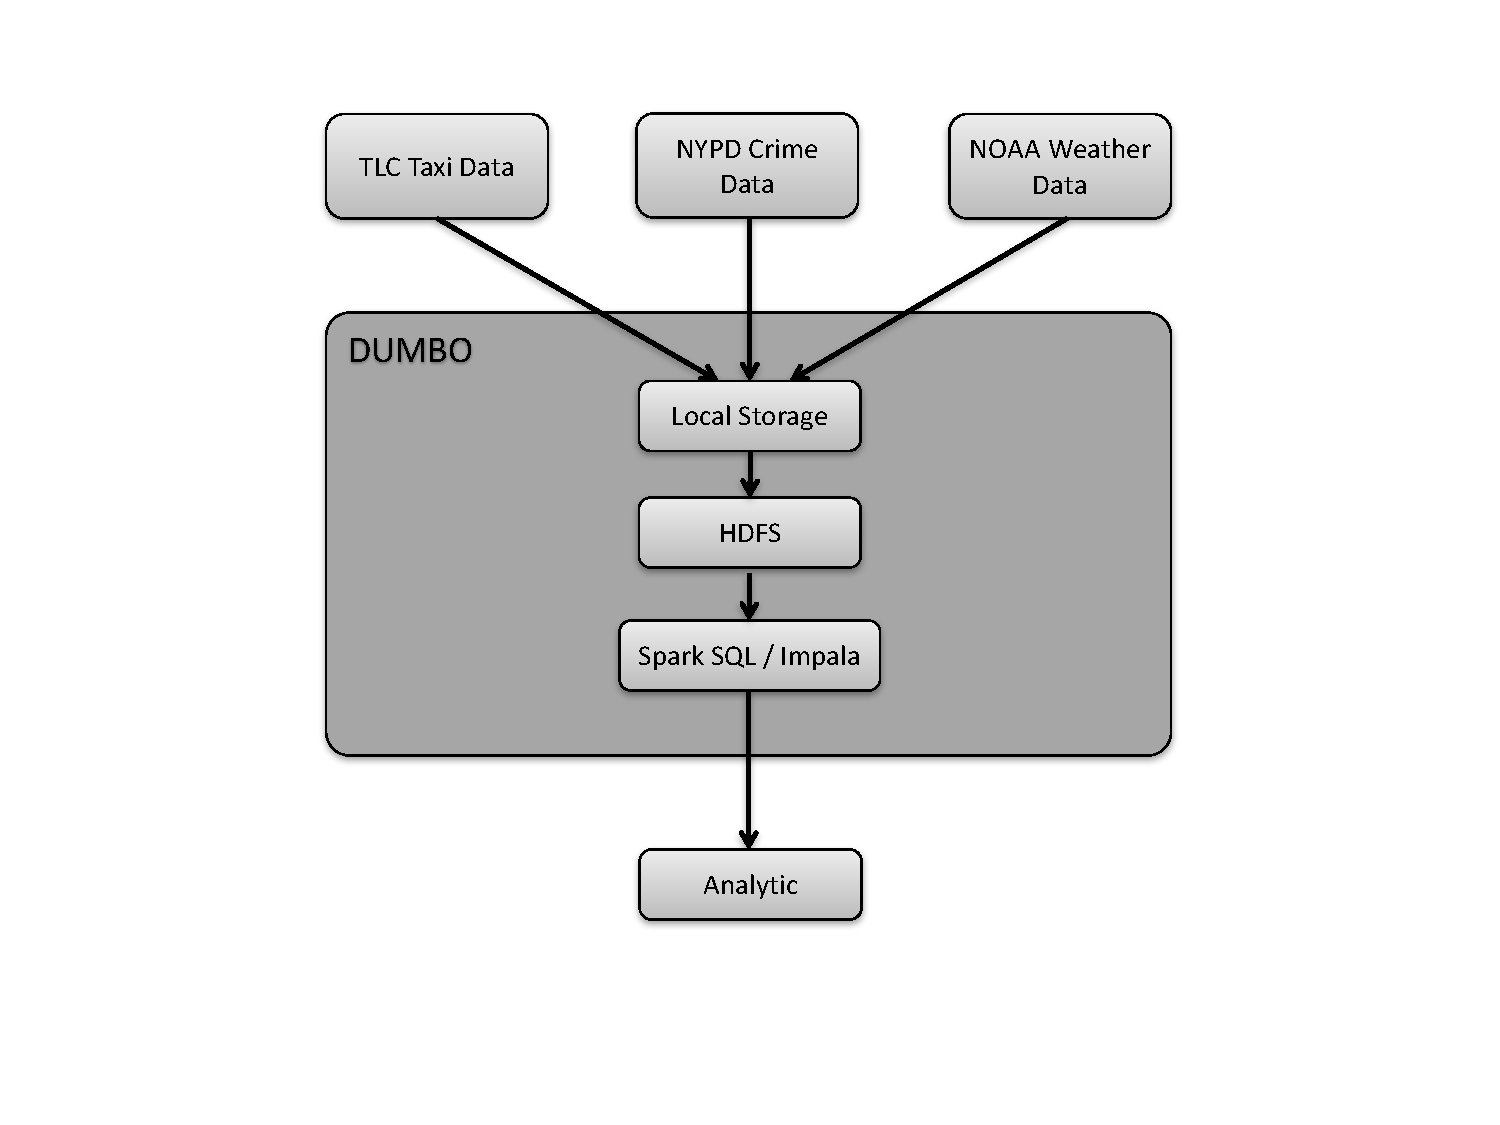
\includegraphics[width=.5\textwidth]{DesignFlowDiagram.pdf}
\end{figure}


% \subsection{Tables}
% ...

% \subsection{Theorem-like Constructs}
% ....


%%%%%%%%%%%%%%%%%%%%%%%%%%%%%%%%%%%%%%%%%%%%%%%%%%%%%%%%%%
% CONCLUSIONS
%%%%%%%%%%%%%%%%%%%%%%%%%%%%%%%%%%%%%%%%%%%%%%%%%%%%%%%%%%

% \section{Conclusions}
% This paragraph will end the body of this sample document.
% Remember that you might still have Acknowledgements or
% Appendices; brief samples of these
% follow.  There is still the Bibliography to deal with; and
% we will make a disclaimer about that here: with the exception
% of the reference to the \LaTeX\ book, the citations in
% this paper are to articles which have nothing to
% do with the present subject and are used as
% examples only.
%\end{document}  % This is where a 'short' article might terminate



%%%%%%%%%%%%%%%%%%%%%%%%%%%%%%%%%%%%%%%%%%%%%%%%%%%%%%%%%%
%ACKNOWLEDGEMENTS are optional
%%%%%%%%%%%%%%%%%%%%%%%%%%%%%%%%%%%%%%%%%%%%%%%%%%%%%%%%%%
% \section{Acknowledgments}
% This section is optional; it is a location for you
% to acknowledge grants, funding, editing assistance and
% what have you.  In the present case, for example, the
% authors would like to thank Gerald Murray of ACM for
% his help in codifying this \textit{Author's Guide}
% and the \textbf{.cls} and \textbf{.tex} files that it describes.



%%%%%%%%%%%%%%%%%%%%%%%%%%%%%%%%%%%%%%%%%%%%%%%%%%%%%%%%%%
% REFERENCES
%%%%%%%%%%%%%%%%%%%%%%%%%%%%%%%%%%%%%%%%%%%%%%%%%%%%%%%%%%
% ACM needs 'a single self-contained file'! SO WE'll NEED TO CHANGE THIS AT THE END.
\bibliographystyle{abbrv}
\bibliography{biblio} 



%%%%%%%%%%%%%%%%%%%%%%%%%%%%%%%%%%%%%%%%%%%%%%%%%%%%%%%%%%
% APPENDIX
%%%%%%%%%%%%%%%%%%%%%%%%%%%%%%%%%%%%%%%%%%%%%%%%%%%%%%%%%%
%APPENDICES are optional
% \balancecolumns
% \appendix
% %Appendix A
% \section{Headings in Appendices}


\end{document}
